% =====================================================================
%  Section 5: Experiments  (his verified Sec. 5 plus, from the previous
%  Overleaf: the common protocol, fuller instance descriptions, and the
%  closed-form validation of Theorem thm:infeasible.  Labels kept.)
% =====================================================================
\section{Experiments}
\label{sec:exp}

\noindent\textbf{Instances.}
\emph{Adult} income classification \cite{uci_adult}: logistic regression
($d{=}109$ with intercept, cross-entropy, $\eta{=}0.1$) on $100$
race-homogeneous groups of $30$ samples, the number of groups per race
proportional to its prevalence (White/Black/Asian-Pac./Amer-Ind./Other
$=85/10/3/1/1$); the importance target is the fairness target itself, $1/5$
per race divided equally among its groups, so a group from the smallest
race carries $p_i=0.2$. \emph{IMDb-Wiki} age regression
\cite{rothe2018imdbwiki}: linear regression of age on $128$-d ResNet face
embeddings ($\eta{=}10^{-2}$) over the first $100$ identities with $30$
images, with the cubic importance target $p_i\propto(101-i)^3$.
Observation rates are swept through a one-parameter family: on Adult
$r\propto p^{\beta}$, $\beta\in\{0,\tfrac14,\tfrac12,\tfrac34,1\}$, from
uniform observation (prevalence regime, $\nu{=}.60$: the five groups of the
three smallest races hold $60\%$ of the target against $r_i\approx K/m$)
to importance-aligned ($\nu{=}0$); on IMDb-Wiki $r_i\propto i^{\beta}$,
$\beta\in\{0,\tfrac12,1,\tfrac32,2,3\}$, from uniform observation
($\nu{=}.31$, nine groups) to the mirror image of $p$ ($\nu{=}.88$, $41$
groups), plus the aligned $r_i\propto 101-i$ ($\nu{=}0$). Eleven instances,
$\nu$ from $0$ to $.88$.

\noindent\textbf{Protocol.}
Each step observes $K{=}3$ groups drawn without replacement with
probabilities $\propto r$, which induces $q$ over the $\binom{100}{3}$
compositions; $q$ is estimated from $10^6$ draws of the sampler and the plan
from \eqref{eq:ipfp} on the membership mask, once per instance. Each
observed group takes $H{=}5$ local steps on its own data before the weighted
average, the standard practical deviation from the one-step analysis,
applied to every rule alike since all rules consume the same local updates
from the same draw $A^t$. Rules: \avot{}; \emph{group-blind averaging}, the
uniform average over the observed groups (Proposition~\ref{prop:surrogate}
with $\tilde p_i=r_i/K$); the \emph{fixed multiplier} $m/K$, the rescaling
$(m/K)\,p_i$ that presumes uniform observation; and \emph{full}, every group
every step weighted by $p$, the reference $\Phi(p)$. Stepsize
$\eta_t=\eta/(1+t/1000)$ unless stated, fixed before the comparison and
shared by every rule; across nine schedules (constant, hyperbolic with
$T_0\in\{250,\dots,16000\}$, inverse square root, step, cosine) the winner
never changes on any instance, only the margin does: a faster decay puts
full coverage on its floor and widens the IMDb-Wiki gap (cosine: $84.12$
against $90.69$), a constant stepsize narrows it to a tie. $4000$ steps, $5$
seeds; we report $F_p$ averaged over the last $500$ steps, mean $\pm$ std
over seeds. On both
instances $\argmin F_w$ is available to machine precision (closed form for
least squares, Newton for the logistic loss), so the floors
$\Phi(p),\Phi(\hat p),\Phi(\tilde p)$ of Theorem~\ref{thm:infeasible} are
exact rather than estimated, and in every instance with $\nu=0$ the
iteration \eqref{eq:ipfp} converges to a row error below $3\cdot10^{-8}$,
certifying the remaining inequalities of \eqref{eq:hall}.

% ----------------------------------------------------------- Table 1
\begin{table}[t]
\centering
\caption{Headline cells, tail-500 over $5$ seeds, decaying stepsize. \emph{full}
sees every group every step; \emph{upsamp.}, self-normalized upsampling
(weights $\propto p_i/r_i$ within the batch); LDS, label-distribution
smoothing \cite{yang2021dir}, regression only. The fixed multiplier $m/K$
diverges whenever observation rates are non-uniform.}
\label{tab:overall}
\footnotesize\setlength{\tabcolsep}{2.2pt}
\begin{tabular}{lcccccc}
\toprule
Instance & \avot{} & unif.\ avg & upsamp. & LDS & $m/K$ & full \\
\midrule
Adult, $\nu{=}.60$ & $\best{0.2269}$ & $0.2479$ & $0.2288$ & -- & $0.670$ & $0.2073$ \\
Adult, $\nu{=}0$   & $0.2075$ & $0.2077$ & $0.2075$ & -- & div. & $0.2073$ \\
IMDb, $\nu{=}.31$  & $\best{86.06}$ & $91.63$ & $86.74$ & $94.28$ & $8504$ & $82.95$ \\
IMDb, $\nu{=}0$    & $\best{84.28}$ & $86.37$ & $84.40$ & $89.43$ & div. & $82.95$ \\
\bottomrule
\end{tabular}
\end{table}

% ----------------------------------------------------------- Fig 2
\begin{figure}[t]
\centering
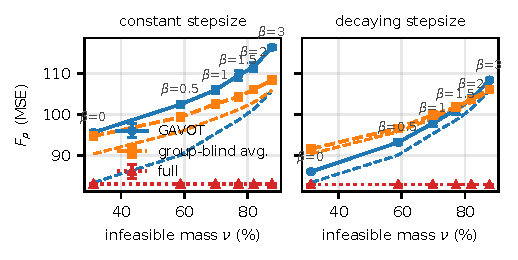
\includegraphics[width=0.92\columnwidth]{figs/severity_imdb.pdf}
\caption{IMDb-Wiki severity sweep. Solid, measured tail-500 ($\pm1$ std);
dashed, the exact floor $\Phi(\cdot)$ each rule converges to. Left, constant
stepsize: the optimization residual swamps the alignment gain and transport
loses everywhere, even where the floors are seven units apart. Right, decaying
stepsize: the residual collapses and the measured curves track their floors, so
transport wins until the floors close at high $\nu$. The sign is set by which of
the two terms of \eqref{eq:infeasible} dominates, not by the regime label.}
\label{fig:severity}
\end{figure}

\begin{figure}[t]
\centering

\includegraphics[width=0.99\columnwidth]{figs/rare_group_adult.pdf}\\[2pt]
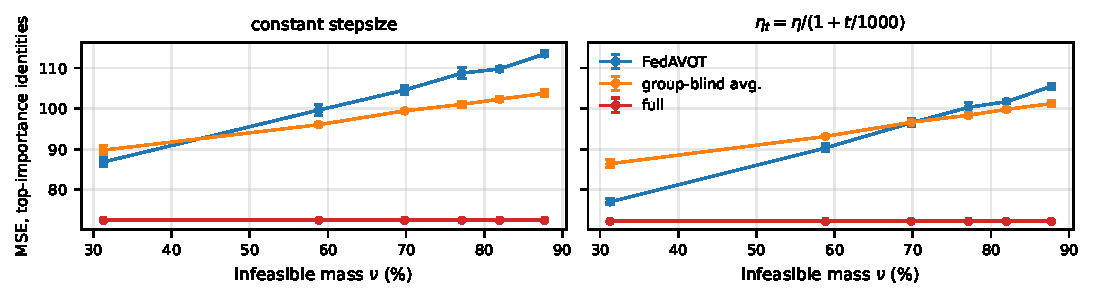
\includegraphics[width=0.99\columnwidth]{figs/rare_group_imdb.pdf}
\caption{Loss on the least represented group, the metric the fairness target
is about. Top, Adult: cross-entropy on race Other, one group of $30$ out of
$100$, to which the category-uniform target assigns $p_i=0.2$; the axis is
the observation-rate exponent, $\beta{=}1$ aligned, $\beta{=}0$ uniform
(prevalence). Bottom, IMDb-Wiki: MSE on the $20$ highest-importance
identities, the least observed ones once $\beta>0$, against $\nu$. Left
panels constant stepsize, right panels decaying. Same protocol as the
tables ($K{=}3$, $H{=}5$, $4000$ steps, tail-500 mean $\pm$ std over $5$
seeds); lower is better. Curves are the group-wise entries of the same runs
as Table~\ref{tab:overall} and Fig.~\ref{fig:severity}.}
\label{fig:rare}
\end{figure}

\noindent\textbf{The least represented group.}
Fig.~\ref{fig:rare} reads the same runs on the group the target exists for.
On Adult, transport lowers the loss on race Other at every skew and under
both stepsizes: $.073$ against $.119$ for group-blind averaging on the
prevalence instance (full coverage $.031$), and $.031$ against $.035$ on the
aligned one, where it matches full coverage. Amer-Indian, the other
single-group race, behaves the same way. On IMDb-Wiki the top-importance
identities show the crossover of Table~\ref{tab:severity} one step earlier:
under decay transport wins at $\nu\le.70$ ($77.0$ against $86.4$ at
$\nu{=}.31$, full $72.2$; $73.6$ against $79.9$ when aligned) and loses at
the three most infeasible skews, while at constant stepsize it wins only at
$\nu{=}.31$. The single most starved group, the one with the largest
$p_i/r_i$ in each instance, sharpens the picture: on Adult it is race Other
itself ($p_i/r_i{=}6.7$); on IMDb-Wiki it is the top identity, where under
decay transport gives $253$ against $331$ at $\nu{=}.31$ and $373$ against
$380$ at $\nu{=}.59$ (full $219$), then loses from $\nu{=}.70$ on, the same
crossover one step earlier still (a $30$-image group, so $\pm5$ to $10$
across seeds). The overall objective and the rare-group loss therefore tell
the same story, with the rare group the more sensitive of the two.

\noindent\textbf{Why transport stops helping.}
The failure is not a bug of the weights; it is the two terms of
\eqref{eq:infeasible} changing sign. A starved group has $p_i>r_i$, so the
plan can deliver at most $r_i$ of its mass: past the coverage law of
Cor.~\ref{cor:batchsize} the reachable target $\hat p$ truncates at the
observation rate, and as $\nu$ grows $\hat p$ and the group-blind $\tilde p$
starve the same groups, so the two floors converge (Table~\ref{tab:severity},
$\Delta_{\mathrm{floor}}$ from $6.99$ to $0.02$). What transport still does
is concentrate weight on the starved group whenever it does appear, $p_i/r_i$
times its batch share, which is exactly the variance Lemma~\ref{lem:variance}
does not see: the second moment is bounded, the variance about the mean is
not, and it is largest on the rare group. Once the floors coincide that
variance is all that separates the two rules, so transport loses by the
residual, by $2$ to $8$ at constant stepsize and by $2.3$ at $\nu{=}.88$ even
under decay. Transport helps exactly while there is mass left to move.

\noindent\textbf{E1: the headline cells.}
Table~\ref{tab:overall} reports the four instances a practitioner would
recognize. Transport wins on three: Adult under prevalence-proportional
availability, $0.2269$ against $0.2479$ ($t{=}45$), and both IMDb cells,
$86.06$ against $91.63$ ($t{=}21$) and $84.28$ against $86.37$ ($t{=}13$). On
Adult with importance-aligned availability the two coincide at the oracle
value, which is what Proposition~\ref{prop:surrogate} predicts when
$\tilde p=p$: there is nothing to correct and transport does not manufacture a
difference. The fixed multiplier diverges on both aligned instances and is far
off on the other two, so naive rescaling is no alternative to solving \eqref{eq:mot}.
Two imbalance baselines sit between the two. Self-normalized upsampling
(weights $\propto p_i/r_i$, renormalized within the batch), the reweighting
form of oversampling rare groups, recovers most of the gain and transport
the rest: $0.2288$ against $0.2269$ on Adult prevalence ($t{=}5.8$) and
$86.74$ against $86.06$ on IMDb skewed ($t{=}2.6$, at the margin of
significance with $5$ seeds); on the aligned instances the two coincide, as
every convex rule must. Downsampling ($\min(p_i/r_i,1)$, normalized) is never
better than upsampling ($0.2308$, $86.90$). Label-distribution smoothing
\cite{yang2021dir}, the standard imbalanced-regression correction, reweights
by the rarity of the label value rather than by how rarely a group is
observed, and trails even group-blind averaging on both IMDb-Wiki instances
($94.28$, $89.43$). On the least represented group the margin of transport
over upsampling widens: $77.0$ against $80.0$ at $\nu{=}.31$ and $73.6$
against $75.6$ when aligned on IMDb-Wiki, $.073$ against $.075$ on Adult
prevalence. Upsampling is the one-shot heuristic for the marginal problem
\eqref{eq:mot} solves exactly, without the feasibility certificate or the
floor decomposition.

% ----------------------------------------------------------- Table 2
\begin{table}[t]
\centering
\caption{IMDb-Wiki severity sweep, decaying stepsize. $\Delta_{\mathrm{floor}}$
is the alignment gain of Theorem~\ref{thm:infeasible}, \emph{gain} the measured
advantage of transport, $t$ its Welch statistic (population std). The excess
residual transport pays averages $1.9$, and the sign flips exactly where
$\Delta_{\mathrm{floor}}$ crosses it. The five Adult skews all sit above their
crossover and are omitted.}
\label{tab:severity}
\setlength{\tabcolsep}{3.0pt}
\begin{tabular}{ccccc}
\toprule
$\beta$ & $\nu$ & $\Delta_{\mathrm{floor}}$ & gain & $t$ \\
\midrule
$0$   & $.31$ & $6.99$ & $\best{+5.57}$ & $20.7$ \\
$0.5$ & $.59$ & $5.71$ & $\best{+3.46}$ & $11.3$ \\
$1.0$ & $.70$ & $3.67$ & $\best{+2.05}$ & $5.4$ \\
$1.5$ & $.77$ & $2.56$ & $+0.58$ & $1.1$ \\
$2.0$ & $.82$ & $1.62$ & $-0.03$ & $-0.1$ \\
$3.0$ & $.88$ & $0.02$ & $-2.28$ & $-7.9$ \\
\bottomrule
\end{tabular}
\end{table}

\noindent\textbf{E2: the crossover, and where the sign comes from.}
Table~\ref{tab:severity} and Fig.~\ref{fig:severity} are the paper's main
evidence. On Adult, whose five skews are omitted from the table, the measured gain tracks
$\Delta_{\mathrm{floor}}$ within $4\%$ at three of five
($.0134$ against $.0129$, $.0050$ against $.0049$, $.0002$ against $.0003$)
and exceeds it at the two most infeasible ($.0210$ against $.0110$, $.0181$
against $.0144$), group-blind averaging sitting further above its floor. On IMDb-Wiki the gain is
uniformly below the floor by an excess optimization residual that is close to
constant in $\beta$, mean $1.9$ in MSE units, and the measured sign flips
precisely where $\Delta_{\mathrm{floor}}$ crosses that value, between
$\beta{=}1.5$ ($2.56$, gain $+0.58$) and $\beta{=}2.0$ ($1.62$, gain $-0.03$).
This is Theorem~\ref{thm:infeasible} read at finite $T$: the sign of the
comparison is a quantity one computes in advance.

\noindent\textbf{E3: the $\ell_1$ bound is too loose to be the criterion.}
The distances $\|p-\hat p\|_1$ and $\|p-\tilde p\|_1$ are also computed on every
instance, and $\|p-\hat p\|_1<\|p-\tilde p\|_1$ holds in all eleven, including
the three where transport loses or ties. The $\ell_1$ form of
Theorem~\ref{thm:infeasible} therefore never predicts a loss and cannot serve as
the criterion; the exact floors can.

\noindent\textbf{E4: the residual is a stepsize artifact.}
The left panel of Fig.~\ref{fig:severity} runs the identical instances at
constant stepsize. There transport loses on all six IMDb skews, by as much as
$7.9$, even at $\nu{=}.31$ where the floors are $6.99$ apart. The transport
weights $Y[\cdot,j]$ concentrate mass on rarely observed groups, so although
Lemma~\ref{lem:variance} bounds the second moment identically for both rules,
the variance about the mean is larger, and at constant stepsize the iterates sit
on a noise floor proportional to it. Under $\eta_t=\eta/(1+t/1000)$ that floor
decays, the measured curves fall onto their dashed floors, and every sign
reversal attributable to the stepsize disappears. The residual is a property of
the schedule, not of the estimator.

\noindent\textbf{E5: the decomposition in closed form.}
The mirrored IMDb-Wiki instance ($\nu{=}.88$) is where
Theorem~\ref{thm:infeasible} can be read off exactly. The Sinkhorn limit
truncates the target at the observation-rate ceiling,
$\hat p_i\approx\min(p_i,r_i)$ up to renormalization (maximum deviation
$.023$), with $\|p-\hat p\|_1=1.58$ of a possible $2$. The frontier is least
squares, so $\Phi(p)=82.9$, matching the measured full plateau $82.95$, and
$\Phi(\hat p)=105.9$: the alignment floor is $23.0$ and the realized bias
equals its exact expression $|(p-\hat p)^\top L(\theta^\dagger)|=30.7$, where
$L$ collects the per-group risks, while the $\ell_1$ form $2M\|p-\hat p\|_1$
is conservative since $M\ge\max_i L_i(\theta^\dagger)\approx 454$.
Group-blind averaging has the same floor to two decimals,
$\Phi(\tilde p)=105.9$: both surrogates starve the same groups, so
$\Delta_{\mathrm{floor}}$ vanishes and the entire measured gap between the
two rules at this endpoint of Table~\ref{tab:severity} is residual, which is
why it is the one instance where transport still loses by a significant
margin under decay ($\beta{=}2$, where the floors are $1.6$ apart, is a tie).

\noindent\textbf{E6: risk aversion, and where it does not help.}
Sweeping $(\alpha,\gamma)$ on a $10\times10$ grid, the overall objective is
minimized on the $\gamma=1$ edge on every instance, which is
$\kappa(1,\gamma)=1$ made visible and confirms that risk aversion costs the
average. The one place the CVaR layer earns its keep is the worst race on Adult
under prevalence availability, where \avotcvar{} at $(0.2,0.7)$ reaches
$0.3624$ against $0.3679$ for \avot{} and $0.3994$ for group-blind averaging.
Per race, transport improves four of five (Black $.179$ vs $.200$, Asian-Pac
$.368$ vs $.399$, Am-Ind $.175$ vs $.189$, Other $.073$ vs $.119$) and regresses
only the majority group ($.339$ vs $.332$), which is what reweighting toward a
category-uniform target is supposed to do.

\noindent\textbf{Why risk aversion does not reach the rare group.}
On the least represented group the CVaR layer never helps: over the whole
$(\alpha,\gamma)$ grid the best rare-group loss is at $\gamma{=}1$, i.e.\ with
the layer switched off, on all four headline instances, and at
$(\alpha,\gamma)=(0.1,0.1)$ it nearly triples the loss on race Other
($.207$ against $.073$) and raises the top-identity loss on IMDb-Wiki from
$77.0$ to $103$. The reason is where the tilt lands. CVaR upweights the
groups whose realized loss exceeds the running threshold, but it can only
tilt among the groups in the batch, and the rare group is absent from most
batches: the extra weight goes to whichever observed group is doing badly
that step, not to the group the target is about. Composed with transport,
the hinge multiplies weights that are already $p_i/r_i$ large, so the
product amplifies the variance of \eqref{eq:infeasible} rather than the
alignment, which is why the loss grows as $\alpha$ shrinks. Risk aversion
changes the functional; it does not change who is observed, and observation
is what the rare group lacks. Transport moves mass toward it whenever it
appears; CVaR cannot, and the one gain it produces, on the worst race above,
comes from tilting among the groups that are present.

% =====================================================================
